\begin{center}
  \scalebox{0.885}{
    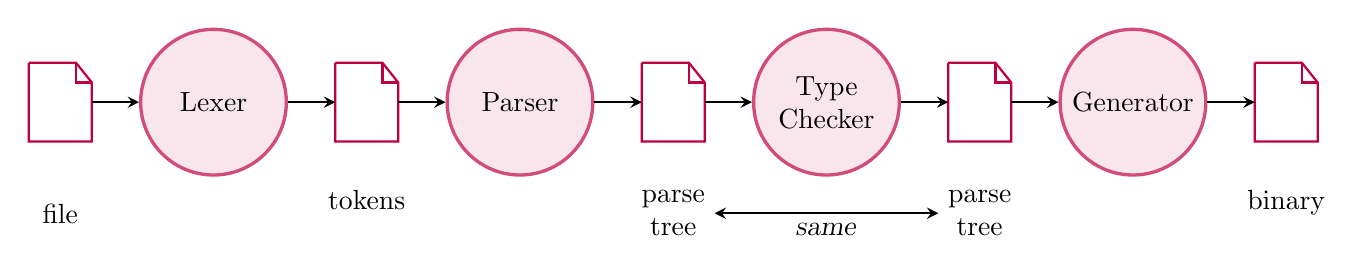
\begin{tikzpicture}[remember picture]
      \newcommand{\spacing}[0]{ 10mm }
      \newcommand{\filesize}[0]{ 0.5 }
      \tikzstyle{edge}  = [thick,>=stealth,draw=black]
      \tikzstyle{dedge} = [thick,->,>=stealth,draw=black]
      \tikzstyle{node}=[
        circle,
        draw=purple!70,
        fill=purple!10,
        anchor=west,
        align=center,
        very thick,
        minimum size=1.85cm
      ]
      \tikzstyle{label}=[
        anchor=north,
        align=center,
      ]
      
      \tikzset{
        pics/file/.style args={#1}{
          code={
            \newcommand{\fileh}[0]{1.0}
            \newcommand{\filew}[0]{0.8}
            \newcommand{\filehc}[0]{\fileh/2}
            \newcommand{\filewc}[0]{\filew/2}
            \draw[-,thick]
              (-\filew *#1, \fileh *#1) to % north west
              ( \filewc*#1, \fileh *#1) to % north east 1
              ( \filew *#1, \filehc*#1) to % north east 2
              ( \filew *#1,-\fileh *#1) to % south east
              (-\filew *#1,-\fileh *#1) to % south west
              (-\filew *#1, \fileh *#1)    % north west
              ;
            \draw[-,thick]
              ( \filewc*#1, \fileh *#1) to
              ( \filewc*#1, \filehc*#1) to
              ( \filew *#1, \filehc*#1)
              ;
          }
        },
      }
      
      % ordinary nodes
      
      \node[node] (lexer)     at (0,0) {Lexer};
      \node[node] (parser)    at ([xshift=2*\spacing]lexer.east) {Parser};
      \node[node] (checker)   at ([xshift=2*\spacing]parser.east) {Type\\Checker};
      \node[node] (generator) at ([xshift=2*\spacing]checker.east) {Generator};
      
      % file nodes
      
      \draw[draw=purple] ([xshift=-\spacing]lexer.west) pic{file={\filesize}};
      \node[label] () at ([xshift=-\spacing,yshift=-2*\filesize*1cm]lexer.west) {\csharp\\file};
      
      \draw[draw=purple] ([xshift=\spacing]lexer.east) pic{file={\filesize}};
      \node[label] () at ([xshift=\spacing,yshift=-2*\filesize*1cm]lexer.east) {tokens};
      
      \draw[draw=purple] ([xshift=\spacing]parser.east) pic{file={\filesize}};
      \node[label] (ptI) at ([xshift=\spacing,yshift=-2*\filesize*1cm]parser.east) {parse\\tree};
      
      \draw[draw=purple] ([xshift=\spacing]checker.east) pic{file={\filesize}};
      \node[label] (ptII) at ([xshift=\spacing,yshift=-2*\filesize*1cm]checker.east) {parse\\tree};
      
      \draw[draw=purple] ([xshift=\spacing]generator.east) pic{file={\filesize}};
      \node[label] () at ([xshift=\spacing,yshift=-2*\filesize*1cm]generator.east) {binary};
      
      % edges
      
      \draw[dedge] ([xshift=-6mm]lexer.west)--(lexer);
      \draw[dedge] (lexer)--([xshift=6mm]lexer.east);
      
      \draw[dedge] ([xshift=-6mm]parser.west)--(parser);
      \draw[dedge] (parser)--([xshift=6mm]parser.east);
      
      \draw[dedge] ([xshift=-6mm]checker.west)--(checker);
      \draw[dedge] (checker)--([xshift=6mm]checker.east);
      
      \draw[dedge] ([xshift=-6mm]generator.west)--(generator);
      \draw[dedge] (generator)--([xshift=6mm]generator.east);
      
      % same parse tree
      \draw[dedge,<->] (ptI) to[edge node={node [below] {\textsl{same}}}] (ptII);
    \end{tikzpicture}
  }
\end{center}
